%!TEX root=../oi-magistr-si.tex
\section[AOS - Kompozice služeb]{Webové služby, automatická kompozice služeb. Orchestrace a choreografie, web mash-up. Modelování služeb a procesů (BPMN, BPEL).}

Na kompozitní službu se můžeme dívat jako na sadu služeb, které spolu spolupracují za účelem vykonání určitého procesu, který definuje interakční workflow. \textbf{Orchestrace} a \textbf{choreografie} jsou rozdílné vzory pro vytváření kompozice služeb. Jazyky pro popis vykonávaného procesu (a tedy i pro popis spolupráce služeb) jsou např. BPMN, BPEL, UML.

\subsection{Orchestrace}
Při tomto přístupu je centrální prvek, který koordinuje všechny zapojené služby. Tento centrální prvek může být také webová služba. Zúčastněné služby nevědí, a ani nemusí vědět, že jsou účastníky nějakého většího procesu, o tom ví jen centrální prvek. Iterakce při orchestraci nastávají na úrovni zpráv.

\subsection{Choreografie}
U choreografie není centrální prvek procesu, a proto všechny zapojené služby ví, kdy volat a s kým dalším spolupracovat. \hl{V praxi se více využívá \textbf{orchestrace}}, protože se díky centrálnímu prvku lépe zotavuje z chyb (chyby jsou odchytávány na jednom místě).

\begin{figure}[h!]
\centering
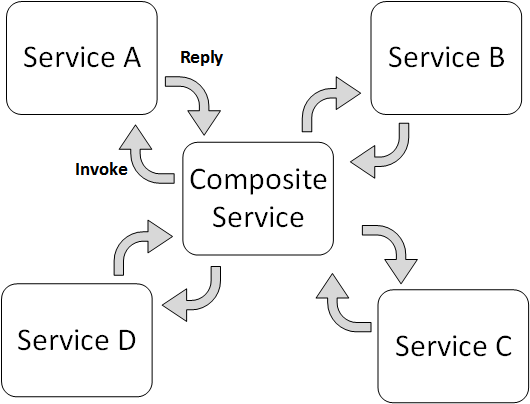
\includegraphics[width=60mm]{11/images/orche}
\hspace{10px}
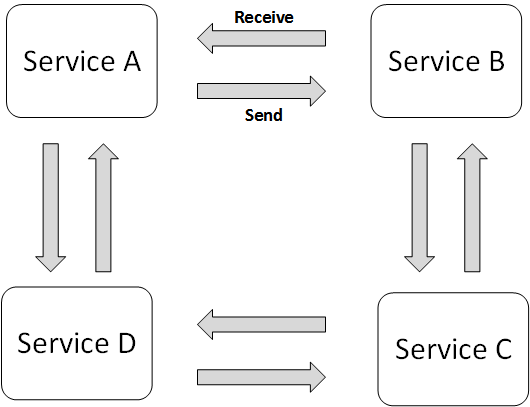
\includegraphics[width=60mm]{11/images/choreo}
\caption{Orchestrace vs. choreografie}
\end{figure}

\subsection{Mashup}
\noindent \hl{Aplikace kombinující data/funkcionalitu z 2 a více zdrojů.}

\begin{itemize}[itemsep=0px,topsep=-2px]
\item Client-based - všechny data se z více služeb volají z klientova prohlížeče (problém s javascriptem Same-Origin Security Policy - POST dotazy).
\item Server-based - Prostředník v podobě serveru, uživatel se dotazuje na jeden server, a ten za něj získává data z ostatních služeb.
\end{itemize}

\subsection{Modelovací jazyky BPMN, BPEL}

\paragraph{BPMN (Business process modeling notation)} Grafická reprezentace pro specifikaci byznys procesu. Podobné UML. Poskytuje mapování mezi grafickou notací a BPEL.

\paragraph{BPEL} \hl{Definice obchodního procesu pomocí jazyka založeného na standardu XML.} BPEL nedefinuje grafické znázornění procesů, ale standardizuje jeho XML definici. BPEL je jazyk pro popis WS kompozice.

\begin{figure}[h!]
\centering
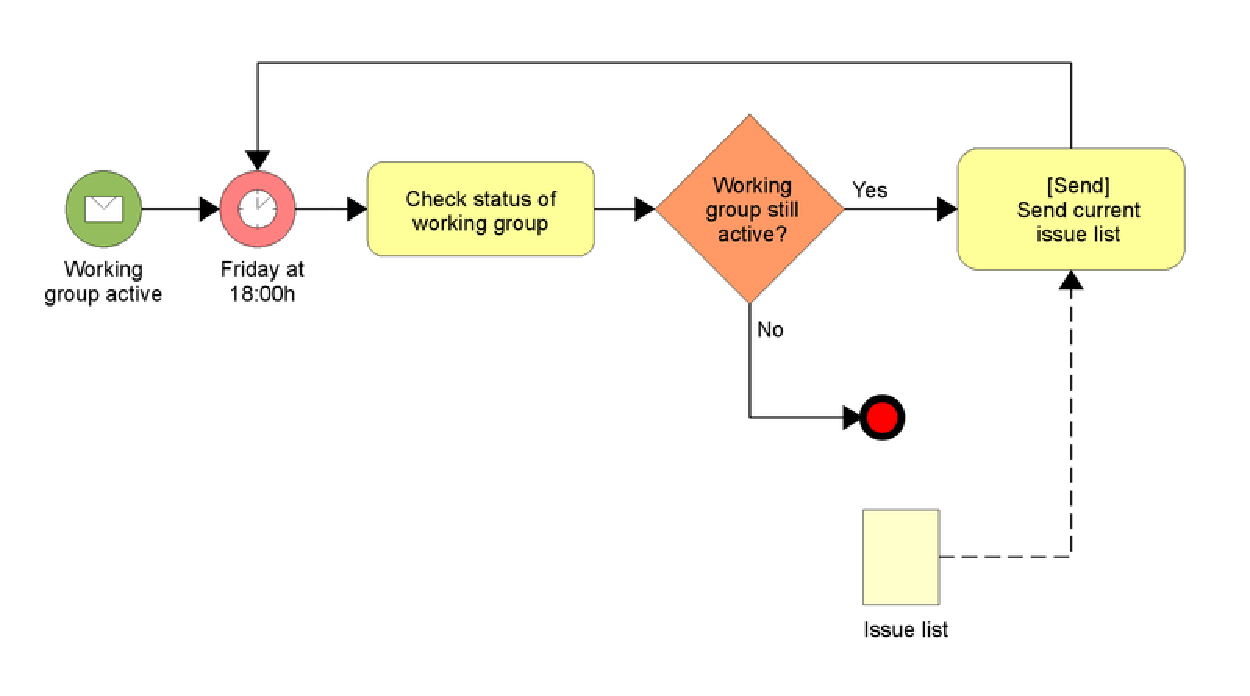
\includegraphics[width=70mm]{11/images/bpmn}
\hspace{10px}
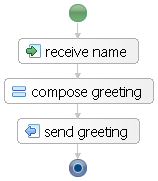
\includegraphics[width=30mm]{11/images/bpel}
\caption{BPMN diagram (pravý diagram je popisován v BPEL kódu)}
\vspace{-10px}
\end{figure}

\lstset{style=xml,caption=BPEL,basicstyle=\scriptsize\ttfamily,label=listing:bpel}
\lstset{language=XML}
\begin{lstlisting}
<process name="HelloWorld" targetNamespace="http://jbpm.org/examples/hello"
  xmlns:tns="http://jbpm.org/examples/hello"
  xmlns:bpel="http://schemas.xmlsoap.org/ws/2003/03/business-process/"
  xmlns="http://schemas.xmlsoap.org/ws/2003/03/business-process/">

  <partnerLinks>
    <!-- establishes the relationship with the caller agent -->
    <partnerLink name="caller" partnerLinkType="tns:Greeter-Caller" myRole="Greeter" />
  </partnerLinks>

  <variables>
    <!-- holds the incoming message -->
    <variable name="request" messageType="tns:nameMessage" />
    <!-- holds the outgoing message -->
    <variable name="response" messageType="tns:greetingMessage" />
  </variables>

  <sequence name="MainSeq">
    <!-- receive the name of a person -->
    <receive name="ReceiveName" operation="sayHello" partnerLink="caller" portType="tns:Greeter" variable="request" createInstance="yes" />
    <!-- compose a greeting phrase -->
    <assign name="ComposeGreeting">
      <copy>
        <from expression="concat('Hello:',bpel:getVariableData('request','name'),'!')"/>
        <to variable="response" part="greeting" />
      </copy>
    </assign>
    <!-- send greeting back to caller -->
    <reply name="SendGreeting" operation="sayHello" partnerLink="caller" portType="tns:Greeter" variable="response" />
  </sequence>
</process>
\end{lstlisting}

\begin{centering}
BPMN $\rightarrow$ BPEL $\rightarrow$ Application
\end{centering}